\documentclass[12pt,a4paper,italian]{book}


% numera i subsubsection 1 - 1.1 - 1.1.1 - 1.1.1.1
\setcounter{secnumdepth}{3}

%%%%%%%%%%%%%%%%%%%%%%%%%%%%%%%%%%%%%%
%    Scelta dei package da usare     %
%%%%%%%%%%%%%%%%%%%%%%%%%%%%%%%%%%%%%%

\usepackage[italian]{babel}
\usepackage[utf8]{inputenc}
\usepackage[T1]{fontenc}
\usepackage{amsmath,amsfonts,amssymb,amsthm}
\usepackage{deistesi}
\usepackage{fancyhdr}
\usepackage{multirow}
\usepackage{tabularx}
\usepackage{float}

\usepackage[
   pdftex,
   pdfauthor={Luca Pascucci},
   pdftitle={Integrazione tra Game Engine e Sistemi Multi-Agente},
   pdfsubject={Attività Propedeutica alla Prova Finale},
   bookmarks=true,
   bookmarksopen=true,
   breaklinks=true,
   colorlinks=true,
   linkcolor=black,
   anchorcolor=blue,
   citecolor=blue,
   filecolor=red,
   urlcolor=blue,
   pdfborderstyle={/S/U/W 1}% border style will be underline of width 1pt
]{hyperref}

\urlstyle{same}

\usepackage[final]{listings}
\usepackage[pdftex,dvipsnames]{xcolor}
\usepackage{inconsolata}

\definecolor{mygray}{gray}{0.6}
\definecolor{delim}{RGB}{20,105,176}
\colorlet{myred}{red!60!black}
\colorlet{numb}{red!60!black}

\lstset{
   frame=bt,
   captionpos=b,
   aboveskip=3mm,
   belowskip=3mm,
   showspaces=false,                % show spaces everywhere adding particular underscores; it overrides 'showstringspaces'
   showstringspaces=false,          % underline spaces within strings only
   showtabs=false,
   columns=flexible,
   extendedchars=true,
   basicstyle=\fontsize{10}{10}\ttfamily,
   numbers=left,
   stepnumber=3,
   numberstyle=\tiny\color{gray},
   keywordstyle=\color{blue},
   commentstyle=\color{ForestGreen},
   stringstyle=\color{mygray},
   breaklines=true,
   breakatwhitespace=true,
   tabsize=2,
   title=\lstname,
   literate=
  {á}{{\'a}}1 {é}{{\'e}}1 {í}{{\'i}}1 {ó}{{\'o}}1 {ú}{{\'u}}1
  {Á}{{\'A}}1 {É}{{\'E}}1 {Í}{{\'I}}1 {Ó}{{\'O}}1 {Ú}{{\'U}}1
  {à}{{\`a}}1 {è}{{\`e}}1 {ì}{{\`i}}1 {ò}{{\`o}}1 {ù}{{\`u}}1
  {À}{{\`A}}1 {È}{{\'E}}1 {Ì}{{\`I}}1 {Ò}{{\`O}}1 {Ù}{{\`U}}1
  {ä}{{\"a}}1 {ë}{{\"e}}1 {ï}{{\"i}}1 {ö}{{\"o}}1 {ü}{{\"u}}1
  {Ä}{{\"A}}1 {Ë}{{\"E}}1 {Ï}{{\"I}}1 {Ö}{{\"O}}1 {Ü}{{\"U}}1
  {â}{{\^a}}1 {ê}{{\^e}}1 {î}{{\^i}}1 {ô}{{\^o}}1 {û}{{\^u}}1
  {Â}{{\^A}}1 {Ê}{{\^E}}1 {Î}{{\^I}}1 {Ô}{{\^O}}1 {Û}{{\^U}}1
  {Ã}{{\~A}}1 {ã}{{\~a}}1 {Õ}{{\~O}}1 {õ}{{\~o}}1
  {œ}{{\oe}}1 {Œ}{{\OE}}1 {æ}{{\ae}}1 {Æ}{{\AE}}1 {ß}{{\ss}}1
  {ű}{{\H{u}}}1 {Ű}{{\H{U}}}1 {ő}{{\H{o}}}1 {Ő}{{\H{O}}}1
  {ç}{{\c c}}1 {Ç}{{\c C}}1 {ø}{{\o}}1 {å}{{\r a}}1 {Å}{{\r A}}1
  {€}{{\euro}}1 {£}{{\pounds}}1 {«}{{\guillemotleft}}1
  {»}{{\guillemotright}}1 {ñ}{{\~n}}1 {Ñ}{{\~N}}1 {¿}{{?`}}1
}

\lstset{
  language=Java,
  morekeywords={final}
  moredelim=[il][\textcolor{mygray}]{@}{\ },
  moredelim=[is][\textcolor{mygray}]{\%\%}{\%\%}
}

\lstdefinelanguage{json}{
    comment=[l]{//},
    literate=
      {0}{{{\color{myred}0}}}{1}
      {1}{{{\color{myred}1}}}{1}
      {2}{{{\color{myred}2}}}{1}
      {3}{{{\color{myred}3}}}{1}
      {4}{{{\color{myred}4}}}{1}
      {5}{{{\color{myred}5}}}{1}
      {6}{{{\color{myred}6}}}{1}
      {7}{{{\color{myred}7}}}{1}
      {8}{{{\color{myred}8}}}{1}
      {9}{{{\color{myred}9}}}{1}
      {:}{{{\color{myred}{:}}}}{1}
      {,}{{{\color{myred}{,}}}}{1}
      {\{}{{{\color{delim}{\{}}}}{1}
      {\}}{{{\color{delim}{\}}}}}{1}
      {[}{{{\color{delim}{[}}}}{1}
      {]}{{{\color{delim}{]}}}}{1},
}

\lstdefinelanguage{asl}{
    comment=[l]{//},
    morestring=**[d][\color{myred}]{"},
    keywords={include}
}

\usepackage{xargs}
\usepackage[colorinlistoftodos,prependcaption]{todonotes}
\newcommandx{\unsure}[2][1=]{\todo[linecolor=red,backgroundcolor=red!25,bordercolor=red,#1]{#2}}
\newcommandx{\change}[2][1=]{\todo[linecolor=blue,backgroundcolor=blue!25,bordercolor=blue,#1]{#2}}
\newcommandx{\improvement}[2][1=]{\todo[linecolor=ForestGreen,backgroundcolor=ForestGreen!25,bordercolor=ForestGreen,#1]{#2}}
\newcommandx{\marianiSays}[2][1=]{\todo[linecolor=Orange,backgroundcolor=Orange!25,bordercolor=Orange,#1]{#2}}

\makeatletter

\newcommand\ProcessThreeDashes{\llap{\color{cyan}\mdseries-{-}-}}

%%%%%%%%%%%%%%%%%%%%%%%%%%%%%%%%%%%%%%%%
% Scelta delle dimensioni della pagina %
%%%%%%%%%%%%%%%%%%%%%%%%%%%%%%%%%%%%%%%%

\setlength{\textwidth}{13.5cm}
\setlength{\textheight}{19cm}
\setlength{\footskip}{3cm}
\setlength{\headheight}{15pt}
\oddsidemargin=50pt \evensidemargin=20pt

%%%%%%%%%%%%%%%%%%%%%%%%%%%%%%%%%%%%%%
%  Informazioni generali sulla Tesi  %
%    da usare nell'intestazione      %
%%%%%%%%%%%%%%%%%%%%%%%%%%%%%%%%%%%%%%

\titolo{Integrazione tra Game Engine e Sistemi Multi-Agente}
\laureando{Luca Pascucci}
\annoaccademico{2018--2019}
\sessione{II}
\facolta{CAMPUS DI CESENA\\SCUOLA DI INGEGNERIA E ARCHITETTURA}
\corsodilaurea{Ingegneria e Scienze Informatiche}
\corso{Attività Propedeutica alla Prova Finale}
\relatore{Andrea Omicini}
\correlatorea{Stefano Mariani}


\author{Luca Pascucci}
\title{Integrazione tra Game Engine e Sistemi Multi-Agente}
\date{\today}

%%%%%%%%%%%%%%%%%%%%%%%%%%%%%%%%%%%%%
% Fine Preambolo %
% Inizio tesi %
%%%%%%%%%%%%%%%%%%%%%%%%%%%%%%%%%%%%%%

\begin{document}

%%%%%%%%%%%%%%%%%%%%%%%%%
% inizio prefazione
% pagina del titolo, indice, sommario
%%%%%%%%%%%%%%%%%%%%%%%%%

\frontmatter \maketitle \pagestyle{plain} \tableofcontents

\chapter{Sommario}

Con lo sviluppo della tecnologia per creare ambienti virtuali più realistici, complessi e dinamici sta aumentando l'interesse sulle Game Engine (GE), le quali si rivelano sempre più importanti in numerosi ambiti, permettendo lo sviluppo di applicazioni moderne e videogiochi con relativa facilità.

\medskip

Nell'ambito di ricerca, in particolare nel contesto dei Sistemi Multi-Agente (MAS), sono state recentemente utilizzate come supporto alla definizione dell'ambiente e come mezzo abilitante per la coordinazione.\cite{gamemas-woa2016}

\medskip

In questa attività propedeutica alla tesi si analizzerà lo stato dell’arte attuale delle integrazioni tra MAS e GE, ricercando nuove tecnologie utilizzabili con lo scopo finale di realizzare una prima architettura di integrazione, sviluppata successivamente in fase di tesi, utilizzabile per diversi scenari di associazione e comunicazione tra il mondo delle GE ed il mondo dei MAS, lasciando entrambi separati senza modificare le loro astrazioni e funzionalità.


%%%%%%%%%%%%%%%%%%%%%%%%%
% inizio corpo del documento
%
% sequenze dei vari capitoli
% è consigliato mantenere una struttura logica ben definita per separare i vari capitoli
% si consiglia di reificare tale struttura fisicamente sul file system
%%%%%%%%%%%%%%%%%%%%%%%%%

\mainmatter

% stile della pagina
\pagestyle{fancy} \fancyhead[LE,RO]{\bfseries\thepage}

% inclusione dei capitoli
\chapter{Background}

\subsection{Integrazione}

Sono già presenti esempi di integrazione tra GE e MAS che concentrano la propria attenzione su obiettivi specifici a livello tecnologico, piuttosto che sulla creazione di un'infrastruttura orientata agli agenti basata sul gioco per scopi generici. Per esempio:

\begin{itemize}
    \item QuizMASter \cite{5763564} concentrato sull'astrazione degli agenti collegando gli agenti MAS ai personaggi dei motori di gioco, nel contesto dell'apprendimento educativo
    \item CIGA \cite{ciga} considera sia la modellazione degli agenti che quella dell'ambiente, per agenti virtuali generici in ambienti virtuali
    \item GameBots \cite{gamebots} concentrato sull'astrazione dell'agente, ma considera anche l'ambiente fornendo un framework di sviluppo e un runtime per i test di sistemi multi-agente in ambienti virtuali
    \item UTSAF \cite{utsaf} si concentra sulla modellistica ambientale nel contesto di simulazioni distribuite in ambito militare\footnote{Gli agenti vengono considerati, ma solo come mezzo di integrazione tra diverse piattaforme di simulazione, non nel contesto del GE sfruttato per il rendering di simulazione}
\end{itemize}

Sebbene rappresentino chiaramente esempi di integrazione (parzialmente) riuscita di MAS in GE, i lavori sopra elencati presentano alcune carenze rispetto all'obiettivo che perseguiamo in questo documento.

\smallskip

Solamente CIGA rappresenta un'eccezione che riconosce il divario concettuale tra MAS e GE, e propone soluzioni per affrontarlo (anche se a livello tecnologico). L'unico strato preso in considerazione nel perseguimento dell'integrazione è quello tecnologico - nessun modello, nessuna architettura, nessun linguaggio. All'interno di QuizMASter, UTSAF e GameBot (in una certa misura) l'integrazione è realizzata per specifico obiettivo, e la maggior parte degli approcci fornisce ai programmatori alcune astrazioni per trattare con agenti e ambiente, ma nessuna attenzione viene data alle astrazioni sociali \cite{gamemas-woa2016}.


\section{Situazione iniziale}

I lavori precedentemente svolti, che hanno contribuito alla definizione di questo percorso, utilizzano due approcci nettamente separati per l'integrazione MAS e GE:
\begin{enumerate}
	\item Integrazione delle caratteristiche dei MAS all'interno della GE;
	\item Realizzazione di un middleware, come layer software, per collegare l'ambiente MAS con GE.
\end{enumerate}

\subsection{MAS all'interno di GE} \label{MAS_dentro_GE}

Il primo punto è stato realizzato implementando due modelli tipici dei MAS:
\begin{itemize}
	\item Il modello Beliefs, Desires, Intentions (BDI) per la programmazione degli agenti \cite{amslaurea15657};
	\item Un modello di coordinazione degli agenti tramite spazio di tuple e primitive Linda \cite{amslaurea8424}\cite{amslaurea16100};
\end{itemize}

Il cuore pulsante di entrambi i lavori risiede nell'uso intensivo di un interprete Prolog fatto ad hoc per Unity: UnityProlog \cite{unity_prolog}. Questo interprete dispone di molte funzionalità per estendere l'interoperabilità di Prolog con i GameObject.
Dal momento che è stato progettato per essere usato in maniera specifica con Unity, nasce con delle primitive che permettono di accedere e manipolare GameObject e i relativi componenti direttamente da Prolog. UnityProlog introduce tuttavia alcune limitazioni da tenere bene in considerazione \cite{amslaurea15657}, anche se allo stato attuale è l'unica versione di Prolog del quale è stato dimostrato il corretto funzionamento:
\begin{itemize}
	\item Un interprete per Prolog non sarà mai performante quanto lo può essere un compilatore e questo può rappresentare un problema per simulazioni di MAS piu grandi.
	\item Utilizza lo stack C\# come stack di esecuzione, quindi la tail call optimization non è ancora supportata.
	\item Non supporta regole con più di 10 subgoal, quindi a fronte di una regola complessa con tanti goal da controllare, è necessario frammentare la regola in questione in sotto regole con non più di 10 subgoal per ognuna.
\end{itemize}

\subsection{MAS e GE separati} \label{MAS_GE_separati}

Il secondo percorso si differenzia dal primo per la scelta di lasciare separati GE da MAS realizzando un canale di comunicazione tra i due ambienti. \'E stata introdotta una terminologia per contraddistinguere le entità realizzate sul GE (GameObject) e su MAS (agenti), rispettivamente definite "corpi" e "menti" virtuali. \cite{amslaurea12270}

\medskip

Fondamentalmente un corpo deve eseguire azioni e a seguito di determinati eventi deve trasmettere le proprie percezioni alla mente, mentre la mente deve elaborare le percezioni per decidere quali azioni deve far svolgere al proprio corpo. Per rendere possibile questa comunicazione è stato progettato e implementato un sistema middleware definito secondo il seguente schema.

\begin{figure}[H]
\centering
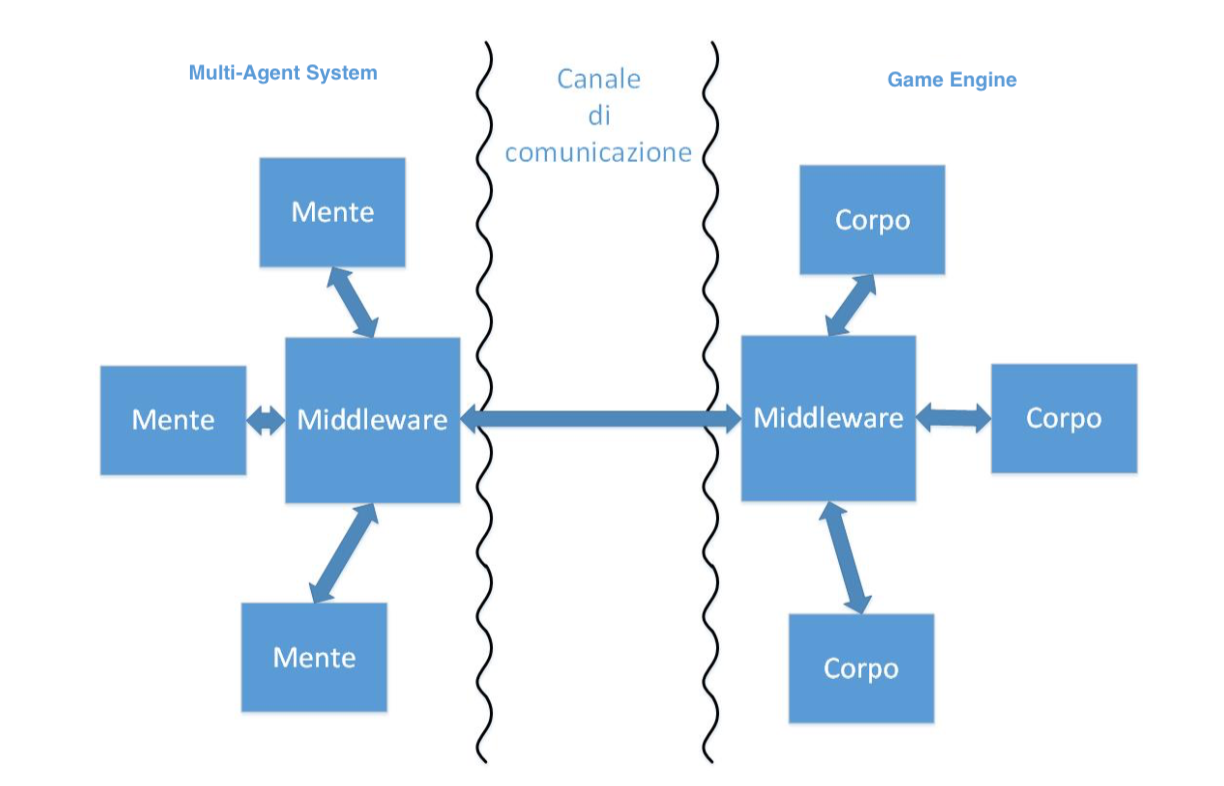
\includegraphics[width=9cm]{figures/Middleware_fuschini.png}
\caption{Il middleware viene suddiviso in due parti, poste sui due lati del canale di comunicazione. \cite{amslaurea12270}}
\end{figure}

Dallo schema si può notare la separazione del middleware nei due sistemi, motivato dalle diverse tecnologie utilizzate dai due ambienti.
Questa divisione vincola la realizzazione di una nuova parte di middleware in caso di utilizzo di un diversa tipologia di GE e/o MAS.
\medskip

Il protocollo di comunicazione tra le entità è stato realizzato utilizzando messaggi strutturati. Da una parte, le menti devono definire quale azione deve compiere il relativo corpo (es. "muoviti in avanti", "ruota", "prendi", ecc.), dall'altro i corpi devono far sapere alle relative menti le proprie percezioni dell'ambiente circostante (es. "mi ha toccato un'entità", "sono alle coordinate 23,12,-6", ecc.).\cite{amslaurea12270}


\subsection{JaCaMo}

JaCaMo è un framework per la programmazione orientata agli agenti che combina tre tecnologie già affermate e sviluppate da diversi anni.

\medskip

Un sistema multi-agente JaCaMo o, equivalentemente, un sistema software programmato con JaCaMo è definito da un'organizzazione Moise di agenti BDI autonomi basati su concetti come ruoli, gruppi, missione e schemi, implementati tramite Jason, che lavorano in ambienti condivisi distribuiti basati su artefatti, programmati in CArtAgO.

\medskip

Ognuna delle tre tecnologie indipendenti che compongono il framework ha il proprio set di astrazioni, modelli di programmazione e meta-modelli di riferimento, per questo motivo in JaCaMo è stato realizzato un meta-modello globale, con l'obiettivo di definire le dipendenze, connessioni, mapping concettuali e le sinergie tra le differenti astrazioni rese disponibili da ogni livello \cite{BOISSIER2013747}.

\begin{figure}[H]
\centering
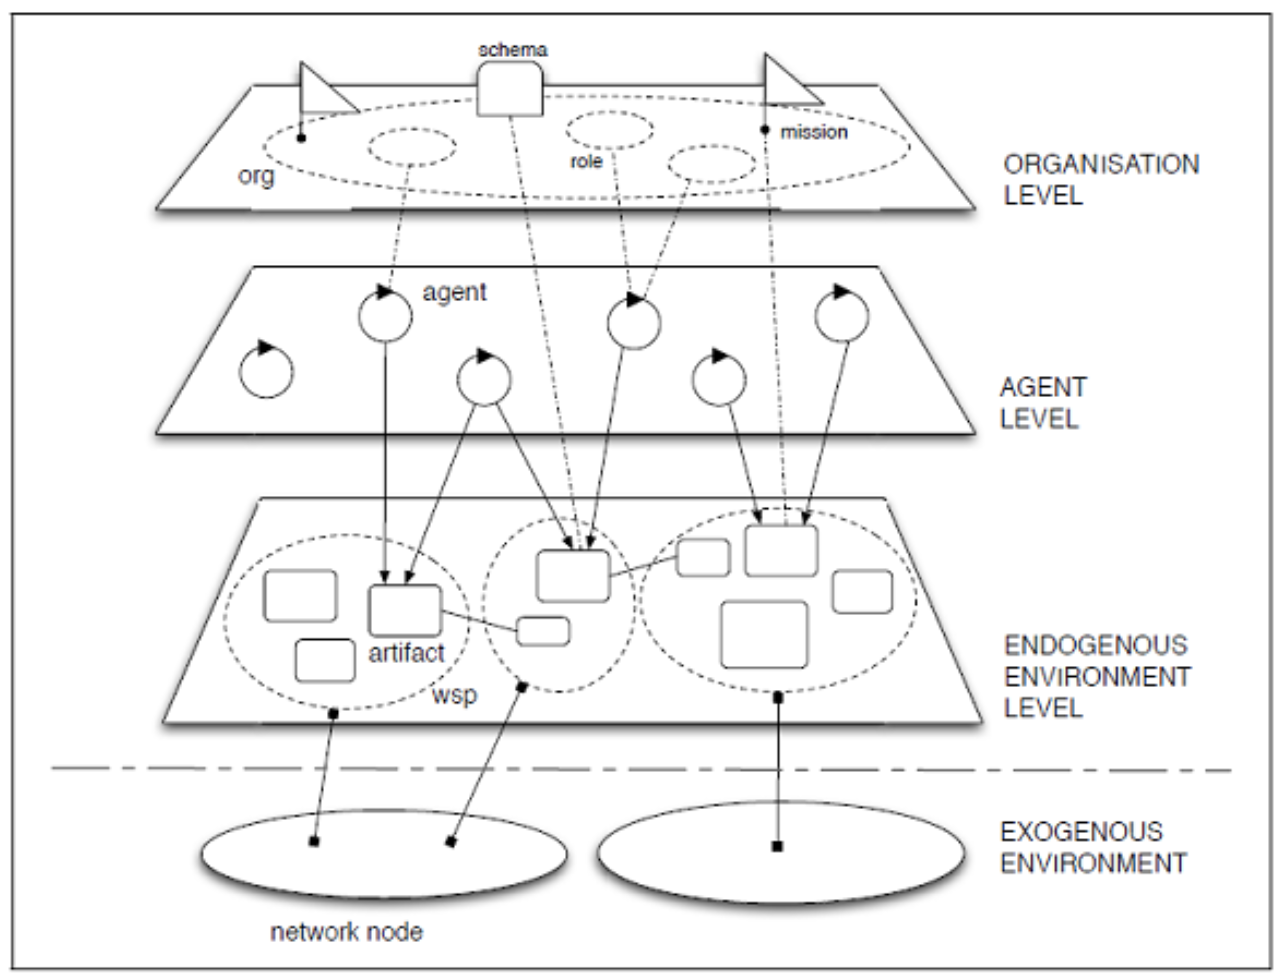
\includegraphics[width=\textwidth]{figures/JaCaMo_levels.png}
\caption{Livelli che compongono il framework JaCaMo \cite{BOISSIER2013747}}
\label{livelli_jacamo}
\end{figure}

\subsubsection{Jason} \label{jason}

Jason è un interprete di AgentSpeak che implementa la semantica operazionale del linguaggio e fornisce una piattaforma di sviluppo per Sistemi Multi-Agente, con molte funzionalità personalizzabili dall'utente.

\medskip

Le astrazioni appartenenti alla dimensione degli agenti, correlate al meta-modello Jason, sono principalmente ispirate all'architettura BDI sulla quale Jason è radicato. Quindi un agente è un'entità composta da un insieme di "beliefs", che rappresenta lo stato corrente e la conoscenza dell'agente sull'ambiente in cui si trova, una serie di "goals", che corrispondono a compiti che l'agente deve perseguire e una serie di "plans" ossia sequenze di azioni (external action or internal action), innescate da eventi, che gli agenti possono comporre, istanziare ed eseguire dinamicamente per compiere i "goals" \cite{jason-book}.

\subsubsection{CArtAgo}
Per quanto riguarda l'ambiente, ciascuna istanza dell'ambiente CArtAgO\footnote{Common ARTifact infrastructure for AGents Open environments} è composta da una o più entità workspace. Ogni workspace è formato da un insieme di artefatti, che forniscono un insieme di operazioni e proprietà osservabili, definendo anche l'interfaccia di utilizzo degli artefatti. L'esecuzione dell'operazione potrebbe generare aggiornamenti delle proprietà osservabili e degli eventi osservabili specifici. L'ultima entità relativa all'ambiente è il “manual”, un'entità utilizzata per descrivere le funzionalità fornite da un artefatto.
Cartago è basato sul meta-modello A\&A (Agents \& Artifacts), che definisce gli agenti come entità computazionali che compiono qualche tipo di attività che mira a uno scopo e gli artefatti come risorse e strumenti costruiti dinamicamente, usati e manipolati dagli agenti per supportare/realizzare le loro attività \cite{cartago}.

\smallskip

\paragraph{Artefatto}
L'artefatto è un'entità reattiva, non autonoma, stateful, riutilizzabile, controllabile ed osservabile. Modellano strumenti, risorse e porzioni di ambiente agendo da strumenti mediatori di azioni e interazioni sociali tra partecipanti individuali e lo stesso ambiente \cite{Omicini2008}.

\begin{figure}[H]
\centering
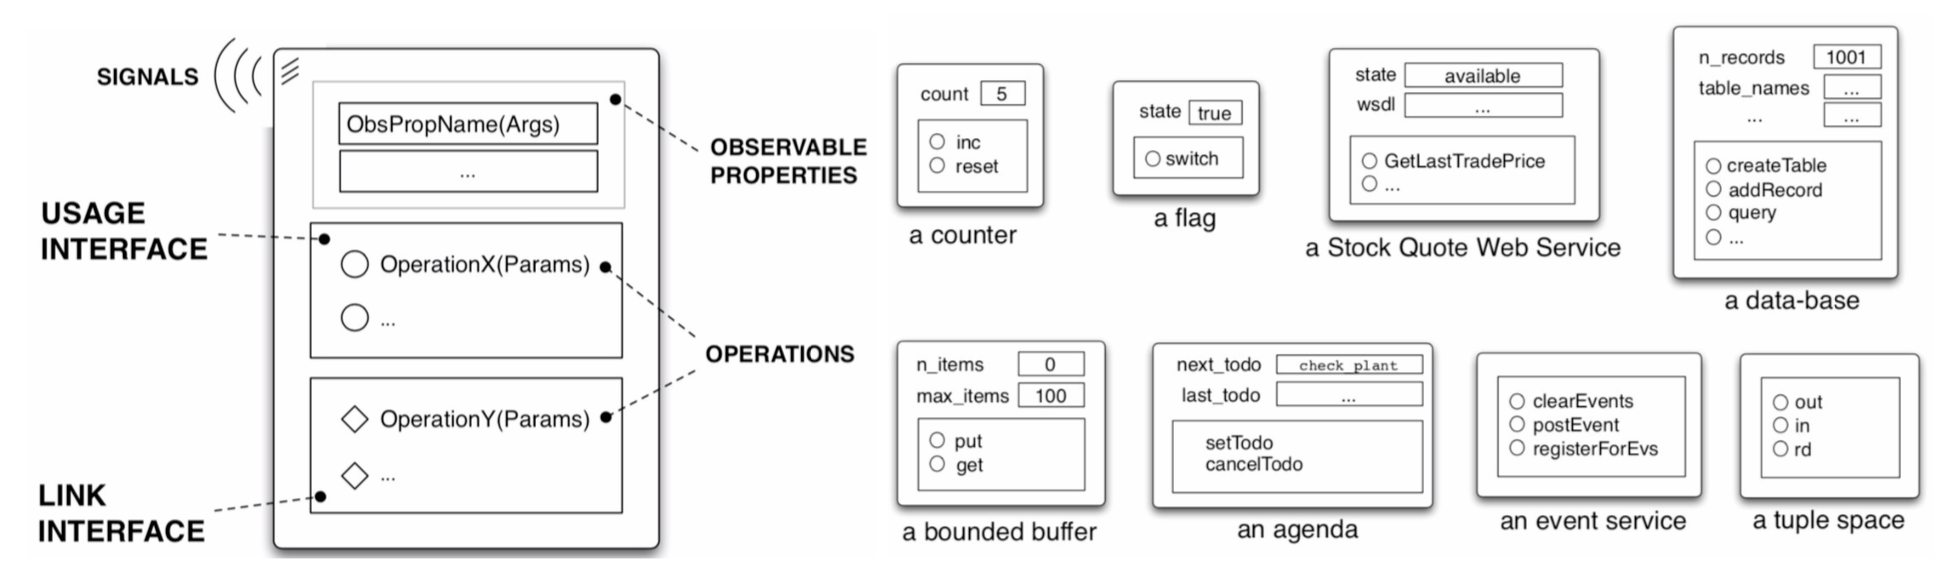
\includegraphics[width=\linewidth]{figures/Artifact_structure_example.png}
\caption{Struttura artefatto con relativi esempi}
\end{figure}

La modalità di interazione tra artefatto ed agente viene riepilogato nell'immagine sottostante.

\begin{figure}[H]
\centering
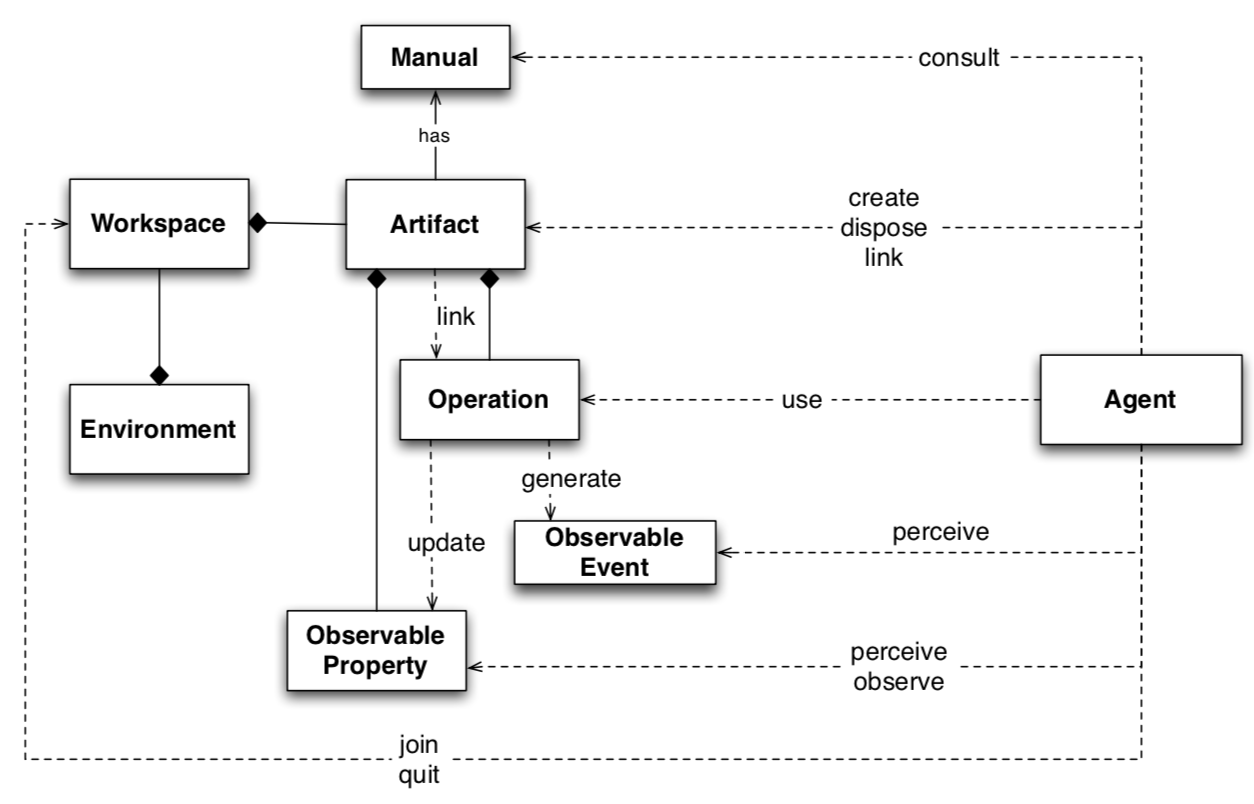
\includegraphics[width=\linewidth]{figures/Artifact_Agent_interaction.png}
\caption{Interazione tra agente ed artefatto}
\end{figure}

\subsubsection{Moise}
Moise è un meta-modello organizzativo per MAS basato sulle nozioni di ruoli, gruppi e missioni. Abilita un MAS ad avere specifiche esplicite per la sua organizzazione. Queste specifiche sono usate sia dagli agenti per ragioni inerenti la loro organizzazione, sia da una piattaforma organizzativa che si assicuri che gli agenti seguano le specifiche.

Moise permette di definire una gerarchia di ruoli con autorizzazioni e missioni, da assegnare agli agenti. Questo permette ai sistemi con un'organizzazione forte, di guadagnare proprietà di apertura (essenzialmente, la proprietà di lavorare con un numero e una diversità di componenti che non è imposta una volta per tutte) e adattamento.



\chapter{Nuova integrazione}


\section{Astrazioni principali}

La situazione attuale di integrazione dei due sistemi presenta dei limiti. Per le motivazioni sopra elencate, in questo elaborato si cerca di definire un'infrastruttura utilizzabile per diversi scenari di associazione e comunicazione tra il mondo delle GE ed il mondo dei MAS, lasciando entrambi separati senza modificare le loro astrazioni e funzionalità.

\medskip

Prima di proseguire con la trattazione è opportuno definire brevemente alcuni concetti che saranno utilizzati da qui in avanti, quali quelli di entità, mente, corpo, azione e percezione. In seguito, verrà quindi proposto uno schema per illustrarne la struttura.

\subsection{Entità}

Con "entità" generalmente viene inteso un insieme di elementi dotati di proprietà comuni dal punto di vista dell’applicazione considerata.\cite{treccani}
Concettualmente, in questo dominio, l'entità viene intesa come oggetto divisibile in due parti, mente e corpo, che collegate riescono a trasmettersi informazioni, utilizzate dalla mente per raggiungere i propri obiettivi e dal corpo per diventare "attivo" nell'ambiente in cui si trova.

\subsection{Mente}

La nozione di "mente" può essere caratterizzata da alcuni punti chiave fondamentali:
\begin{itemize}
   \item autonomia
   \item interazione
   \item obiettivi
\end{itemize}
In altre parole, una mente può essere pensata come un componente software autonomo che interagisce con l'ambiente per svolgere i propri compiti.
I punti sopra elencati rendono facile l'associazione della mente al concetto di Agente, spiegato nella sezione \ref{sistema_multi-agente}, poiché questa entità del Sistema Multi-Agente (MAS) ingloba astrazioni simili a quelle illustrate nella sezione \ref{jason}.

\subsection{Corpo}

"Corpo", poi, è un termine generico che indica qualsiasi porzione limitata di materia, cui si attribuiscono, in fisica, le proprietà di estensione, divisibilità, impenetrabilità.\cite{treccani}
In questa trattazione è associabile alla nozione di GameObject di Unity, spiegata nella sezione \ref{unity}, utilizzata per avere una rappresentazione fisica dell'entità da realizzare.

\subsection{Azione}

Nel suo significato più generale, un'"azione" è intesa come attività od operazione posta in essere da un determinato soggetto.\cite{treccani}
In questo studio, si considera come "azione" un certo gesto richiesto dalla mente che può essere associato ad una operazione eseguita dal corpo, ad esempio, nel
caso di un'azione del tipo \textit{"vai a (posizione)"}, richiesta dalla mente, corrisponde il movimento del corpo nell'ambiente verso la posizione indicata.

\subsection{Percezione}

La "percezione" è un atto cognitivo mediato dai sensi con cui si avverte la realtà di un determinato oggetto e che implica un processo di organizzazione e interpretazione.\cite{treccani}.

\medskip

In questo lavoro, la percezione si collega ad una certa sensazione rilevata dal corpo ed inviata alla mente per portarla a conoscenza di questa nuova informazione, ad esempio, nel caso del raggiungimento della posizione richiesta in precedenza, il corpo trasmette la percezione \textit{"arrivato (posizione)} che informa la mente del completamento dell'operazione.

\medskip

Esiste inoltre, da parte del corpo, la possibilità di inviare percezioni "libere" ossia non associate a risposta di un'azione inviata dalla mente. Un semplice esempio è il contatto del corpo con una qualsiasi altra entità nell'ambiente che corrisponde all'invio di una percezione del tipo \textit{"toccato(nome\_entità)"}.

\subsection{Struttura entità}
Nella figura sottostante viene rappresentata la struttura di una generica entità, dove:

\begin{itemize}
   \item Il corpo esegue azioni e, in risposta a queste ultime, oppure, a seguito di determinati eventi esterni, trasmette le proprie percezioni alla mente.
   \item La mente elabora le percezioni per decidere quali azioni far svolgere al proprio corpo.
\end{itemize}

\begin{figure}[H]
   \centering
   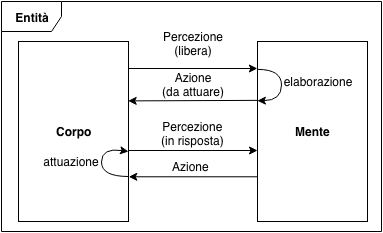
\includegraphics[width=8cm]{figures/Entita_struttura.png}
   \caption{Struttura di una generica entità}
\end{figure}

\section{Stack Tecnologico}

Di seguito vengono illustrate le principali tecnologie prese in esame per la realizzazione di un middleware di collegamento dei due sistemi precedentemente definiti, stabilendo anche quale Sistema Multi-Agente (MAS), Game Engine (GE), framework e tecnologia di collegamento sono stati presi come principale riferimento.

\subsection{JaCaMo}

JaCaMo è un framework per la programmazione orientata agli agenti che combina tre tecnologie già affermate e sviluppate da diversi anni.

\medskip

Un sistema multi-agente JaCaMo o, equivalentemente, un sistema software programmato con JaCaMo è definito da un'organizzazione Moise di agenti BDI autonomi basati su concetti come ruoli, gruppi, missione e schemi, implementati tramite Jason, che lavorano in ambienti condivisi distribuiti basati su artefatti, programmati in CArtAgO.

\medskip

Ognuna delle tre tecnologie indipendenti che compongono il framework ha il proprio set di astrazioni, modelli di programmazione e meta-modelli di riferimento, per questo motivo in JaCaMo è stato realizzato un meta-modello globale, con l'obiettivo di definire le dipendenze, connessioni, mapping concettuali e le sinergie tra le differenti astrazioni rese disponibili da ogni livello \cite{BOISSIER2013747}.

\begin{figure}[H]
\centering
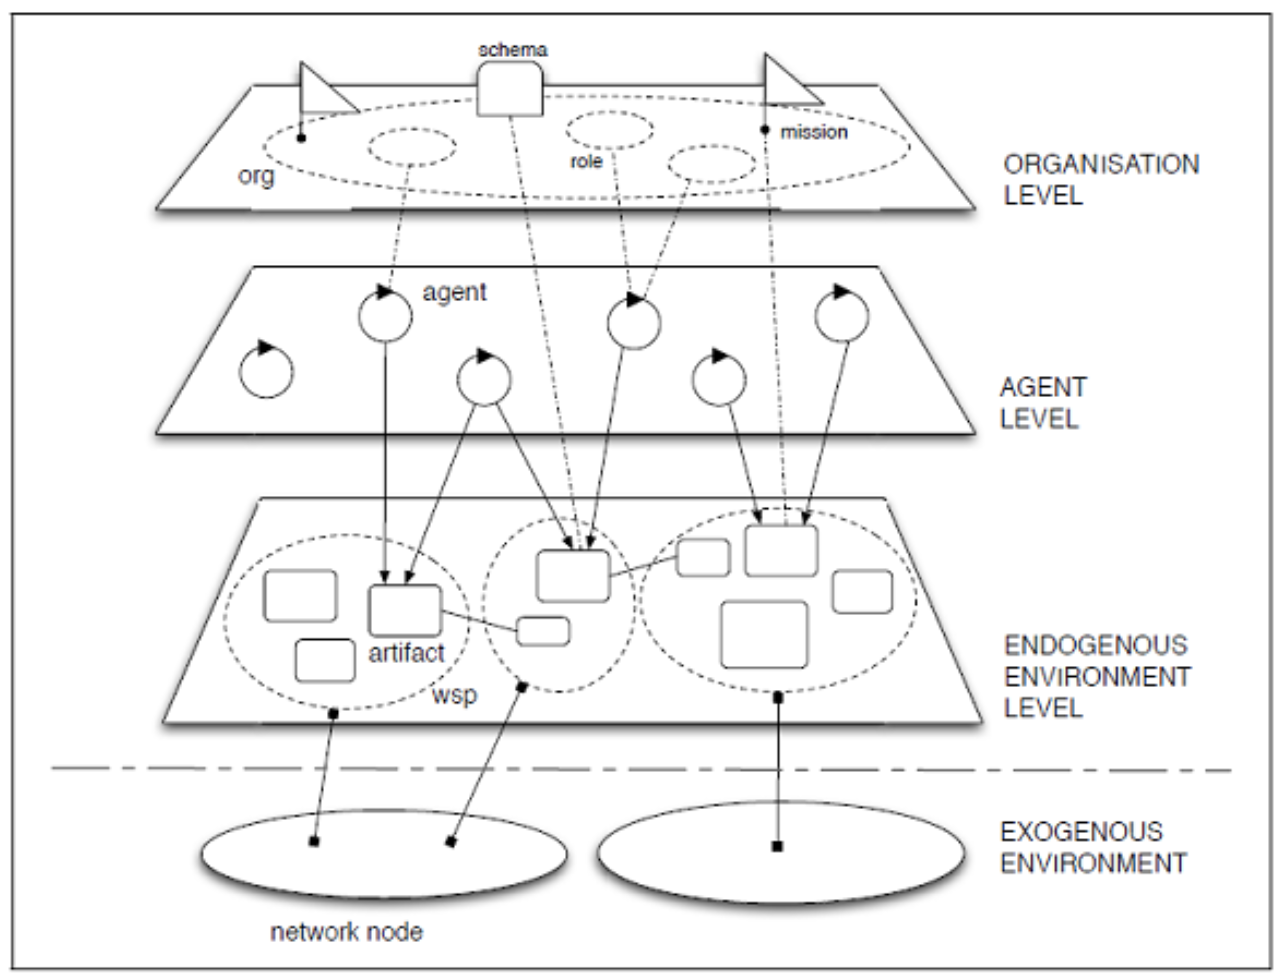
\includegraphics[width=\textwidth]{figures/JaCaMo_levels.png}
\caption{Livelli che compongono il framework JaCaMo \cite{BOISSIER2013747}}
\label{livelli_jacamo}
\end{figure}

\subsubsection{Jason} \label{jason}

Jason è un interprete di AgentSpeak che implementa la semantica operazionale del linguaggio e fornisce una piattaforma di sviluppo per Sistemi Multi-Agente, con molte funzionalità personalizzabili dall'utente.

\medskip

Le astrazioni appartenenti alla dimensione degli agenti, correlate al meta-modello Jason, sono principalmente ispirate all'architettura BDI sulla quale Jason è radicato. Quindi un agente è un'entità composta da un insieme di "beliefs", che rappresenta lo stato corrente e la conoscenza dell'agente sull'ambiente in cui si trova, una serie di "goals", che corrispondono a compiti che l'agente deve perseguire e una serie di "plans" ossia sequenze di azioni (external action or internal action), innescate da eventi, che gli agenti possono comporre, istanziare ed eseguire dinamicamente per compiere i "goals" \cite{jason-book}.

\subsubsection{CArtAgo}
Per quanto riguarda l'ambiente, ciascuna istanza dell'ambiente CArtAgO\footnote{Common ARTifact infrastructure for AGents Open environments} è composta da una o più entità workspace. Ogni workspace è formato da un insieme di artefatti, che forniscono un insieme di operazioni e proprietà osservabili, definendo anche l'interfaccia di utilizzo degli artefatti. L'esecuzione dell'operazione potrebbe generare aggiornamenti delle proprietà osservabili e degli eventi osservabili specifici. L'ultima entità relativa all'ambiente è il “manual”, un'entità utilizzata per descrivere le funzionalità fornite da un artefatto.
Cartago è basato sul meta-modello A\&A (Agents \& Artifacts), che definisce gli agenti come entità computazionali che compiono qualche tipo di attività che mira a uno scopo e gli artefatti come risorse e strumenti costruiti dinamicamente, usati e manipolati dagli agenti per supportare/realizzare le loro attività \cite{cartago}.

\smallskip

\paragraph{Artefatto}
L'artefatto è un'entità reattiva, non autonoma, stateful, riutilizzabile, controllabile ed osservabile. Modellano strumenti, risorse e porzioni di ambiente agendo da strumenti mediatori di azioni e interazioni sociali tra partecipanti individuali e lo stesso ambiente \cite{Omicini2008}.

\begin{figure}[H]
\centering
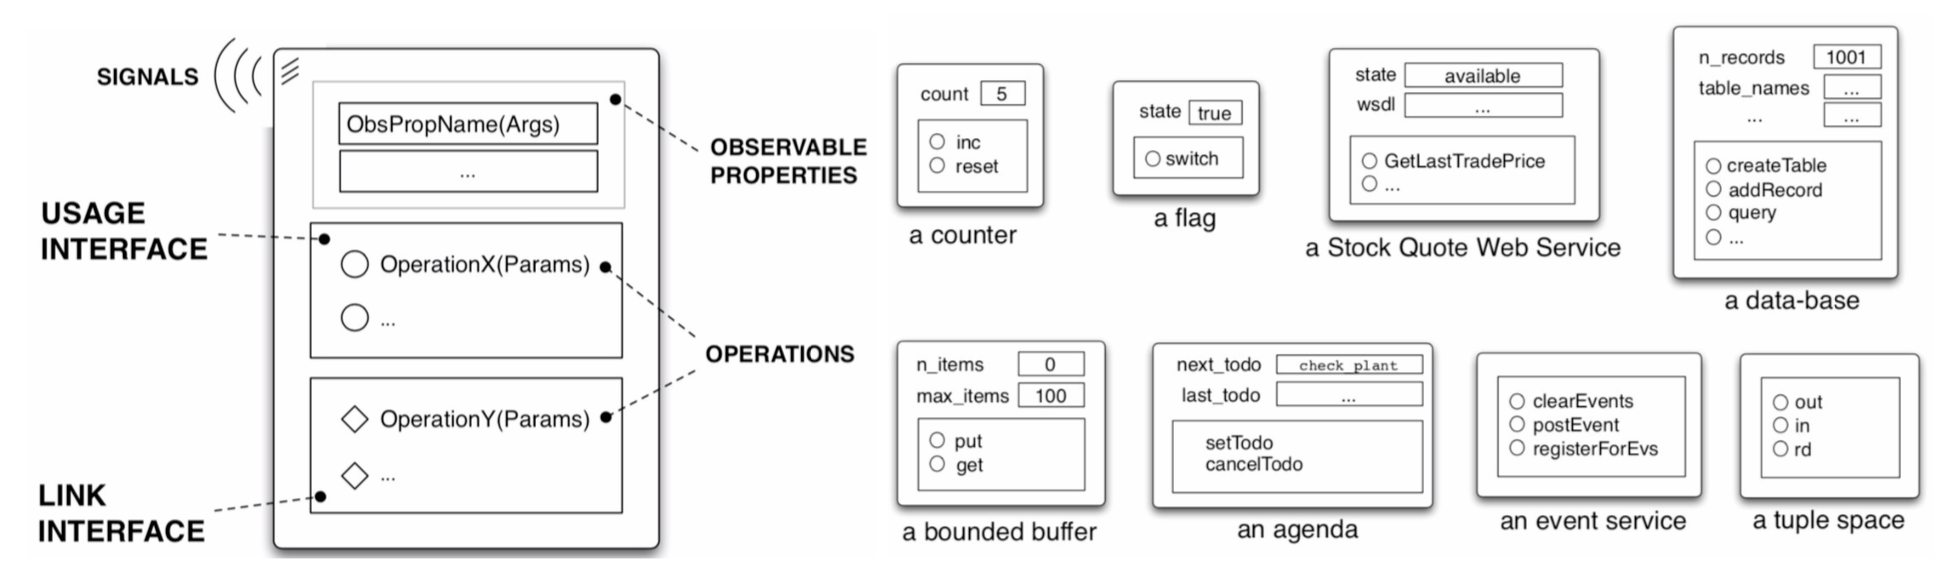
\includegraphics[width=\linewidth]{figures/Artifact_structure_example.png}
\caption{Struttura artefatto con relativi esempi}
\end{figure}

La modalità di interazione tra artefatto ed agente viene riepilogato nell'immagine sottostante.

\begin{figure}[H]
\centering
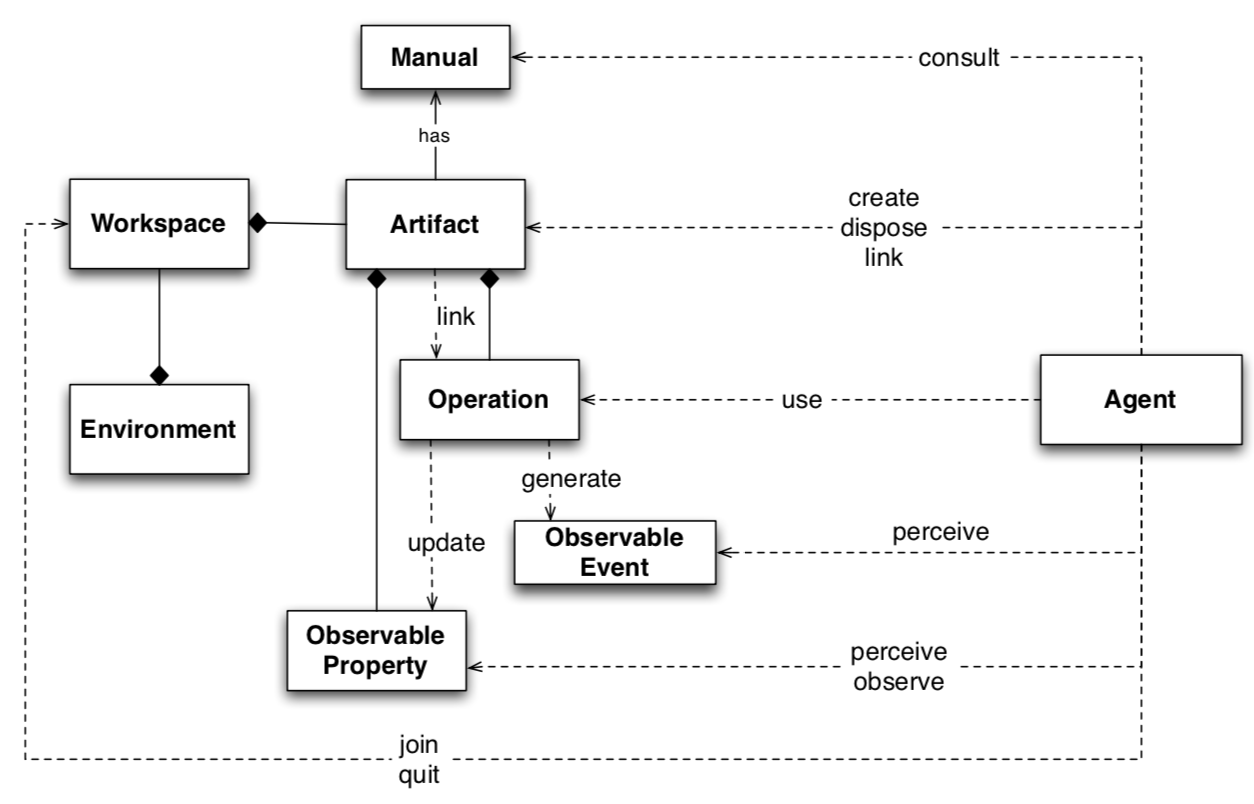
\includegraphics[width=\linewidth]{figures/Artifact_Agent_interaction.png}
\caption{Interazione tra agente ed artefatto}
\end{figure}

\subsubsection{Moise}
Moise è un meta-modello organizzativo per MAS basato sulle nozioni di ruoli, gruppi e missioni. Abilita un MAS ad avere specifiche esplicite per la sua organizzazione. Queste specifiche sono usate sia dagli agenti per ragioni inerenti la loro organizzazione, sia da una piattaforma organizzativa che si assicuri che gli agenti seguano le specifiche.

Moise permette di definire una gerarchia di ruoli con autorizzazioni e missioni, da assegnare agli agenti. Questo permette ai sistemi con un'organizzazione forte, di guadagnare proprietà di apertura (essenzialmente, la proprietà di lavorare con un numero e una diversità di componenti che non è imposta una volta per tutte) e adattamento.


\subsection{Play Framework} \label{play}
Play è un framework lightweight, stateless e asincrono per la creazione di applicazioni e servizi Web. È stato costrutito utilizzando Scala e Akka e mira a fornire gli strumenti per la realizzazione di applicazioni altamente scalabili con consumo minimo di risorse (ad esempio CPU, memoria, thread).\cite{play-framework}

\medskip

Play incorpora un HTTP Server integrato (quindi non è necessario un server di applicazioni Web separato come in molti Web Framework Java), un modello per la realizzazione di applicazioni baste su servizi RESTful e mette a disposizioni strumenti per la gestione di Form, protezione CSRF\footnote{Cross-Site Request Forgery} e meccanismi di instradamento. Per semplificare il suo utilizzo fa largo uso del pattern Model-View-Controller, comune e facilmente utilizzabile, fornendo paradigmi di programmazione concisi e funzionali.

\begin{figure}[H]
\centering
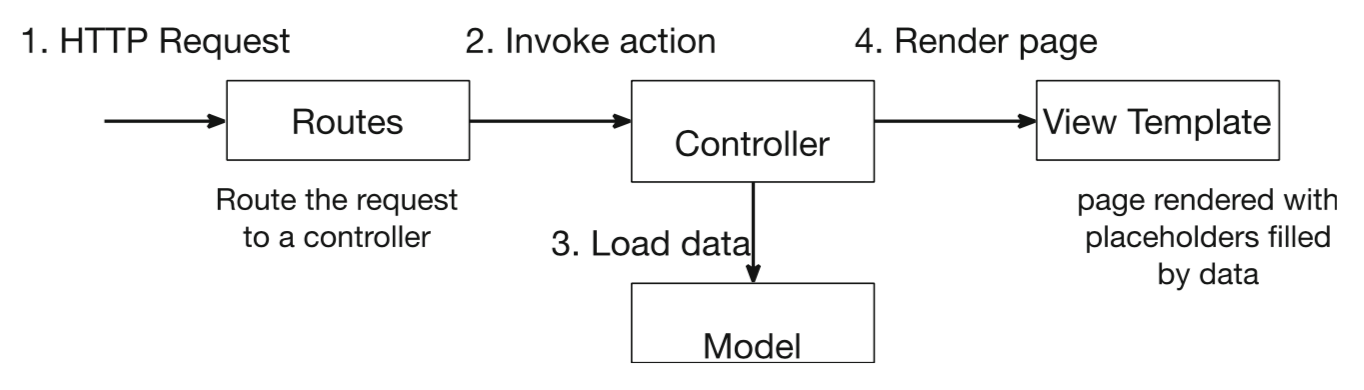
\includegraphics[width=\textwidth]{figures/Play_structure.png}
\caption{Struttura MVC di un'applicazione realizzata con Play\cite{play_framework_book}}
\end{figure}

Lo stack nelle Web Application nel mondo Java Enterprise è basato su una tecnologia che si è evoluta nel corso degli anni e richiede diversi elementi (strati) per funzionare. E' molto probabile che le molteplici tecnologie che comprendono questo stack rendano anche l'implementazione di semplici applicazioni problematica e soggetta a errori poiché ogni tecnologia deve essere integrata con successo con la successiva, spesso basandosi su file di configurazione o convenzioni standard.\cite{play_framework_book}

\begin{figure}[H]
\centering
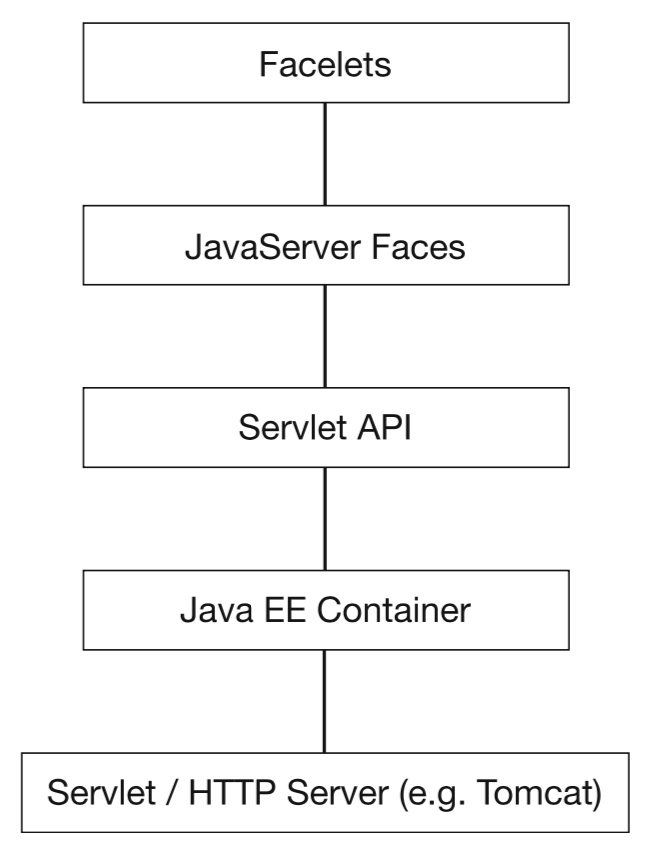
\includegraphics[width=5cm]{figures/Java_EE_layered_architecture.png}
\caption{Architettura a strati JavaEE\cite{play_framework_book}}
\end{figure}

Il framework Play è stato progettato per diminuire lo stack sopra illustrato richiedendo l'utilizzo di un solo server HTTP per funzionare.

\begin{figure}[H]
\centering
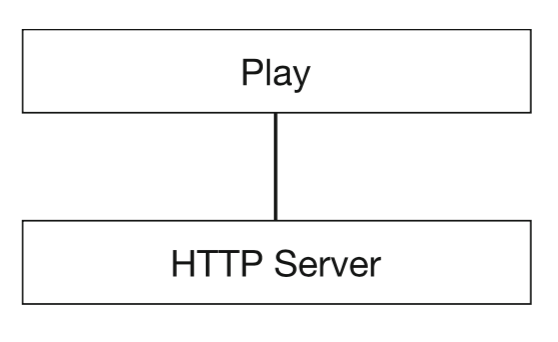
\includegraphics[width=5cm]{figures/Play_layered_architecture.png}
\caption{Architettura a strati Play framework\cite{play_framework_book}}
\end{figure}

Lo strato Play, in figura, è formato da una serie di componenti che includono:
\begin{itemize}
    \item HTTP Server: componente che riceve la richiesta HTTP da un client e restituisce un risultato basato sulle informazioni fornite nella richiesta;
    \item Router: determina dove instradare la richiesta, pertanto fornisce un file di configurazione dei percorsi disponibili nell'applicativo;
    \item Sistema di templating HTML dinamico: Utilizza pagine standard in HTML e le popola con dati generati dinamicamente dall'applicazione;
    \item Console integrata: Per semplificare l'utilizzo di Play, viene fornita una suite di strumenti che possono essere utilizzati per creare, aggiornare e distribuire l'applicazione Play. Questi strumenti sono accessibili e gestiti dalla console;
    \item Persistent framework: Funzionalità utili per accesso a database.
\end{itemize}

Per apprendere al meglio questo framework, dato che non è rientrato tra gli argomenti affrontati durante il corso di studi, sono stati utilizzati il sito \cite{play-framework}, la documentazione \cite{play-framework-documentation} e gli esempi disponibili \cite{play-framework-example}.

\subsubsection*{Akka - Modello ad attori}

Akka è un toolkit per la creazione di applicazioni altamente distribuite, concorrenti, event-driven, tolleranti ai guasti. Play framework utilizza il modello ad attori presente in Akka, dove l'attore è l'entità principale, per aumentare il livello di astrazione e fornire una piattaforma per la realizzazioni di applicazioni simultanee e scalabili \cite{akka}.  Il modello ad attori, all’interno del corso di studi, era già stato illustrato ed utilizzato nell'insegnamento di Sistemi Distribuiti. 

\medskip

Il modello ad attori (che risale al 1973) si basa sull'idea di avere attori simultanei indipendenti che ricevono e inviano messaggi asincroni e che svolgono un comportamento basato su questi messaggi. Gli attori possono mantenere il proprio stato e comportamento. Tuttavia, idealmente solo i dati immutabili vengono scambiati tra di loro, pertanto ogni attore è indipendente da tutti gli altri ed esegue solo alcuni calcoli o elaborazioni basati su un messaggio ricevuto da esso.

\medskip

L'idea chiave alla base del modello ad attori è che la maggior parte dei problemi come concorrenza, deadlock, corruzione dei dati, derivino dalla condivisione dello stato. Pertanto, nel mondo degli attori non esiste uno stato condiviso (come una coda concorrente produttore-consumatore). Al contrario, i messaggi vengono inviati tra attori e questi messaggi vengono messi in coda in una casella di posta in modo simile ai messaggi di posta elettronica. Gli attori rispondono quindi ai messaggi appena arrivano a loro.\cite{play_framework_book}

\begin{figure}[H]
\centering
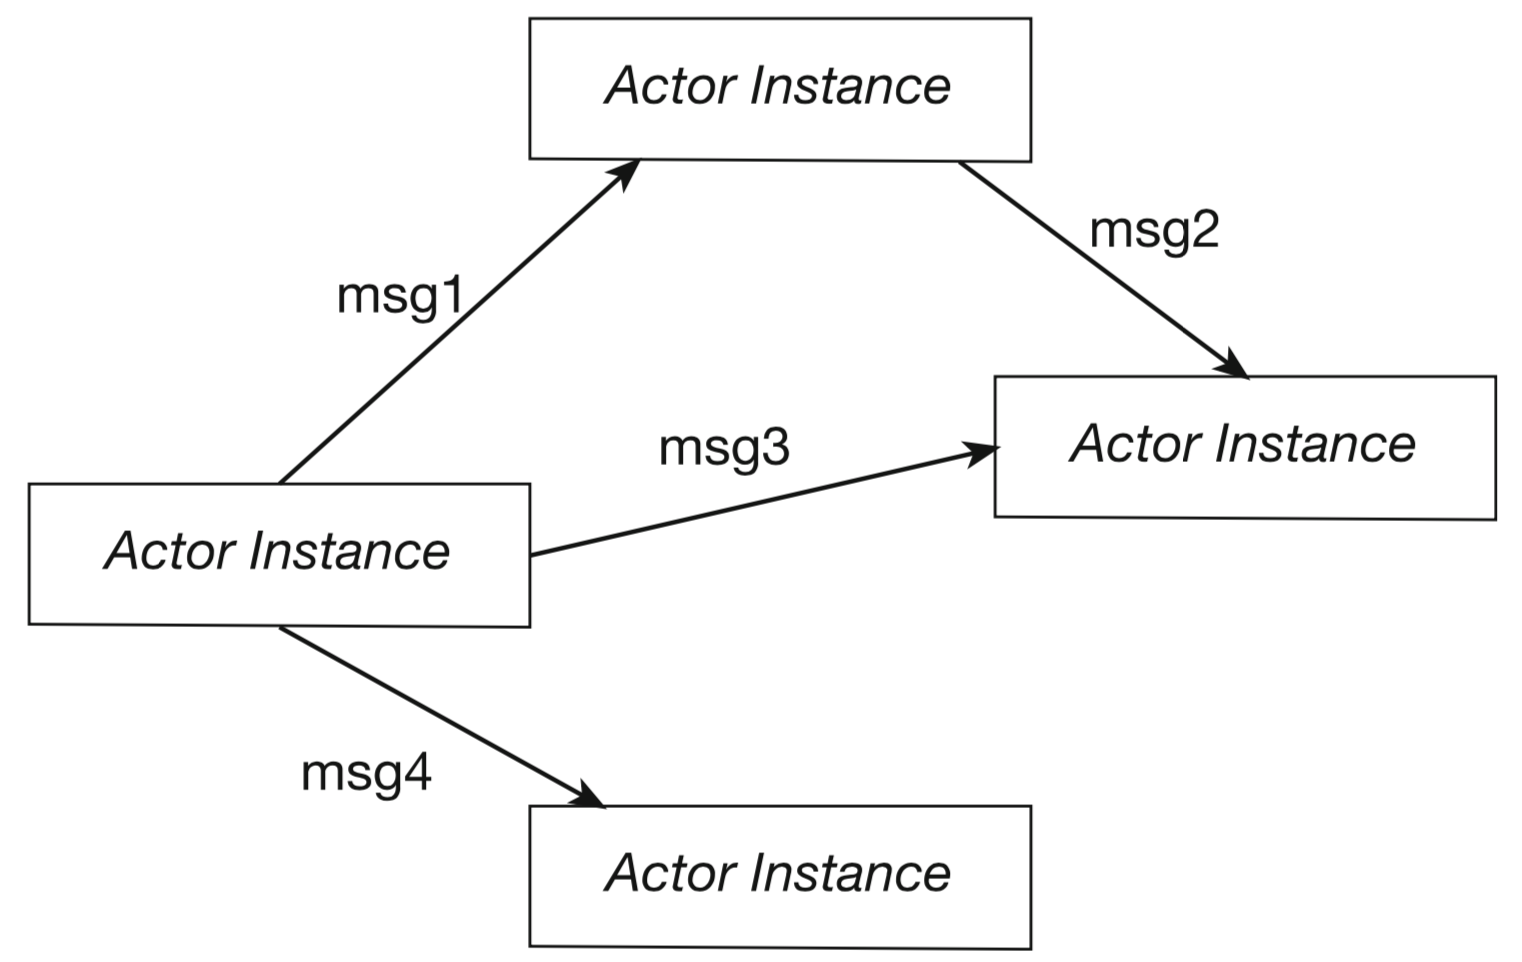
\includegraphics[width=7cm]{figures/Actors_communicating.png}
\caption{Comunicazione tra attori attraverso messaggi asincroni\cite{akka}}
\end{figure}

\subsubsection*{Motivazioni}
Nel presente lavoro è stato utilizzato questo framework perché permette di realizzare un componente separato dal Sistema Multi-Agente e dalla Game Engine, ma allo stesso tempo facilmente collegabile a questi, attraverso richieste HTTP e/o canali WebSocket.

\subsection{WebSocket}

Il protocollo WebSocket (WS) consente la comunicazione bidirezionale tra un client a un host remoto instaurando un canale di comunicazione utilizzabile da entrambi sia in scrittura che in lettura. Il modello di sicurezza utilizzato è l'origin-based security model comunemente usato dai browser web. Il protocollo consiste in una hand-shake di apertura seguita da il successivo invio/ricezione di una serie di messaggi strutturati, stratificata su una connessione TCP\footnote{Transmission Control Protocol} persistente. L'obiettivo di questa tecnologia è fornire un meccanismo per le applicazioni basate su browser che necessitano di comunicazione bidirezionale in tempo reale con server che non si basano sull'apertura di più connessioni HTTP \cite{RFC6455}.
Per comprendere struttura e funzionalità del protocollo WebSocket è stato utilizzato lo standard di riferimento \cite{RFC6455} e le documentazioni delle librerie \cite{websocket-sharp}\cite{tyrus}, entrambe RFC6455 compliant.

\subsubsection*{Introduzione delle WebSocket}

Storicamente, la creazione di applicazioni Web che richiedono la comunicazione bidirezionale tra client e server (ad esempio applicazioni di messaggistica istantanea e giochi) ha portato ad un abuso di HTTP utilizzato per operazioni di polling (verifica ciclica) verso il server con lo scopo di controllare gli aggiornamenti, inviando notifiche upstream come chiamate HTTP distinte \cite{RFC6202}.

\medskip

Il protocollo HTTP è stato inteso fin dalla prima versione ideata da Tim Berners-Lee come metodo per recuperare risorse remote in maniera semplice: una richiesta per ogni pagina Web, ogni immagine o l’invio di dati da rendere persistente. Con il passare degli anni però, all’incirca intorno al 2004, lo sviluppo di applicazioni Web subì una forte accelerazione dovuta all’introduzione di una nuova tecnologia, Ajax, che grazie all'utilizzo di Javascript fu in grado di creare e gestire richieste HTTP asincrone tramite funzioni di callback dedicate.

\medskip

Seguendo l’evoluzione delle applicazioni Web molte applicazioni prevedevano una user experience orientata al real-time. Esempi possono essere applicazioni di chat, videogames multiplayer o sistemi di notifiche, tutte applicazioni che la sola tecnologia Ajax (o simili, come connessioni HTTP persistenti COMET) poteva simulare solo in parte con sistemi di polling poco performanti e complessi da implementare.

\medskip

La soluzione arrivò quando ci si rese conto che la risposta a questi problemi risiedeva effettivamente nel protocollo stesso: HTTP sfrutta a livello di rete il protocollo TCP/IP, connection-oriented, usata in altri contesti singolarmente per connessioni full-duplex. Nacque così il protocollo WebSocket con un ottimo tempismo considerando l’avvento contemporaneo di HTML5 e altre tecnologie dedicate all’open-source che contribuiranno successivamente alla diffusione del protocollo.\cite{websocket_hystory}

\medskip

\subsubsection*{Principali caratteristiche}

Ecco le caratteristiche principali del protocollo WebSocket:
\begin{itemize}
    \item \textbf{Bidirezionali}: quando il canale di comunicazione è attivo, sia il client che il server sono connessi ed entrambi possono inviare e ricevere messaggi;
    \item \textbf{Full-duplex}: i dati inviati contemporaneamente dai due attori (client e server) non generano collisioni e vengono ricevuti correttamente;
    \item \textbf{Basati su TCP}: il protocollo usato a livello di rete per la comunicazione è il TCP, che garantisce un meccanismo affidabile (controllo degli errori, re-invio di pacchetti persi, ecc) per il trasporto di byte da una sorgente a una destinazione;
    \item \textbf{Client-key handshake}: All’apertura di una connessione, il client invia al server una chiave segreta di 16 byte codificata con base64. Il server aggiunge a questa un’altra stringa, detta magic string, specificata nel protocollo (“258EAFA5-E914-47DA-95CA-C5AB0DC85B11”), codifica con SHA1 e invia il risultato al client. Cosi facendo, il client può verificare che l’identità del server che ha risposto corrisponda a quella desiderata;
    \item \textbf{Sicurezza origin-based}: Alla richiesta di una nuova connessione, il server può identificare l’origine della richiesta come non autorizzata o non attendibile e rifiutarla.
    \item \textbf{Maschera dei dati}: Nella trama iniziale di ogni messaggio, il client invia una maschera di 4 byte per l’offuscamento. Effettuando uno XOR bit a bit tra i dati trasmessi e la chiave è possibile ottenere il messaggio originale. Ciò è utile per evitare lo sniffing, cioè l’intercettazione di informazioni da parte di terze parti.
\end{itemize}

\subsubsection*{Motivazioni}
Il protocollo appena illustrato è adatto a far comunicare corpo e mente per la peculiarità di instaurare un canale duraturo e bidirezionale nel quale entrambe le parti possono scambiarsi informazioni (azioni, percezioni). A vantaggio di questa tecnologia sono presenti librerie, ben documentate e realizzate seguendo lo standard RFC6455, facilmente integrabili su JaCaMo e Unity (illustrata nella sezione successiva) e nativamente inserite nel framework Play.

\begin{itemize}
   \item \textbf{websocket-sharp}: Implementazione C\# del protocollo WebSocket client/server\cite{websocket-sharp}
   \item \textbf{project tyrus}: Implementazione Java dello standard JSR 356\footnote{Java API for WebSocket, conforme al protocollo RFC6455}\cite{tyrus}
\end{itemize}


\section{Unity} \label{unity}

Unity è una Game Engine (GE) cross-platform sviluppata da Unity Technologies, utilizzata per la creazione di videogiochi (sia 2D che 3D) e simulazioni, che supporta la distribuzione su una larga varietà di piattaforme (PC, console, dispositivi mobili, etc.). Fornisce astrazioni che contribuiscono ad estendere il suo utilizzo tra gli sviluppatori e programmatori, rendendola una delle GE più utilizzate per produrre in maniera veloce ed efficace applicazioni e giochi.\cite{unity}

\medskip

Inoltre, questa GE supporta molte funzionalità facili da utilizzare e sfruttabili per creare giochi realistici e simulazioni immersive, come un intuitivo editor real-time, un sistema di fisica integrato, luci dinamiche, la possibilità di creare oggetti 2D e 3D (direttamente dall'IDE o di importarli esternamente), gli shader, un supporto per l'intelligenza artificiale (capacità di evitare gli ostacoli, ricerca del percorso, etc.), e cosi via.

\medskip

Le funzionalità principali messe a disposizione del designer sono:
\begin{itemize}
	\item \textbf{GameObject}: La classe base per tutte le entità presenti su una scena di Unity- un personaggio controllabile dall'utente, un personaggio non giocabile, un oggetto (2D/3D). Tutto ciò che è presente sulla scena è dunque un GameObject.
	\item \textbf{Script}: Il codice sorgente applicato a un GameObject, grazie al quale è possibile assegnare a quest'ultimo comportamenti e proprietà dinamiche. Gli script vengono eseguiti dal game loop di Unity che, in maniera sequenziale, esegue una volta ogni script durante ogni frame del gioco. Non esiste concorrenza. Il comportamento è il risultato della logica definita nello script attraverso funzioni e routine. Le proprietà equivalgono a variabili che possono essere valorizzare nello script oppure definite dall'IDE grafico.
	\item \textbf{Component}: Elemento, proprietà speciale assegnabile ai GameObject. A seconda del tipo di GameObject che si desidera creare è necessario aggiungere diverse combinazioni di Component. I Component basilari riguardano la fisica (Transform, Collider,..), l'illuminazione (Light) e la renderizzazione del GameObject (Render). \'E possibile istanziare runtime Components attraverso gli script.
	\item \textbf{Coroutine}: Una soluzione alla sequenzialità imposta agli script, grazie al quale è possibile partizionare una computazione e distribuirla su più frame, sospendendo e riprendendo l'esecuzione in precisi punti del codice.
	\item \textbf{Prefab}: Rappresentazione di un GameObject complesso, completo di Script e Component, istanziabile più volte runtime. Le modifiche della struttura, le proprietà ed i componenti del Prefab si propagheranno a tutti i GameObject collegati allo stesso presenti nella scena di gioco.
	\item \textbf{Event e Messaging System}: sistema ad eventi utile per far comunicare tra loro diversi GameObject. Questi sistemi sono formati tipicamente da eventi e listener. I listener si sottoscrivono ad eventi di un certo tipo: quando l'evento si verifica, viene notificato a tutti i listener dello stesso tipo che sono in ascolto attraverso l'invio di un messaggio.
\end{itemize}

\section{Realizzare un ambiente in Unity} \label{ambiente_unity}

Gli strumenti a disposizione in Unity mettono nelle mani degli sviluppatori la possibilità di realizzare qualunque tipo di oggetto: dai più semplici, come un cubo, ai più articolati, ad esempio un robot. 

\medskip

Per realizzare oggetti complessi è possibile creare una gerarchia di componenti e dotare ognuno di loro delle stesse funzionalità dell'oggetto padre. Ripensando all'esempio del robot, lo sviluppatore può suddividere lo stesso in sotto-componenti più articolate, quali testa, braccia, addome, gambe, fino ad arrivare a realizzare parti basilari quali dita, occhi e così via.

\medskip

Successivamente alla realizzazione dello scheletro dell'oggetto, attraverso la definizione di "script" e l'associazione di "components" è possibile animarlo, dargli una specifica fisicità e renderlo consapevole dell'ambiente che lo circonda. Verranno ora fatti degli esempi per ognuna delle funzionalità appena descritte.

\begin{figure}[H]
\centering
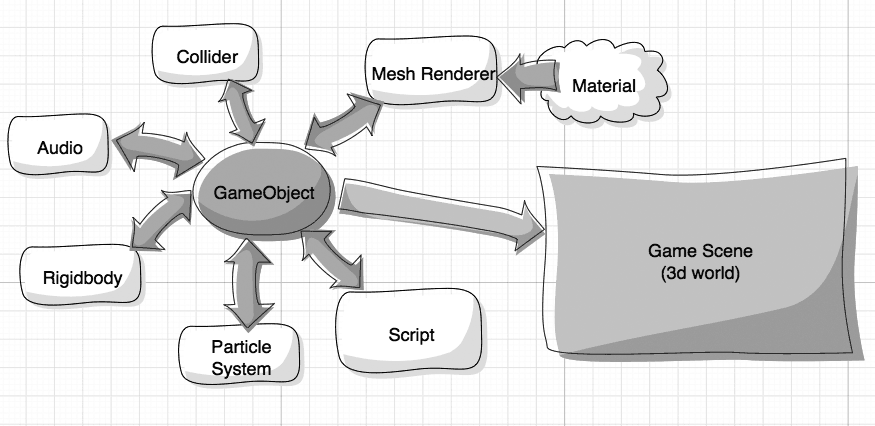
\includegraphics[width=\textwidth]{figures/unity_diagram.png}
\caption{GameObject e Components}
\end{figure}

\subsection{Muovere un GameObject}

Come spiegato precedentemente, ogni oggetto presente su Unity è un GameObject e, per definizione, contiene le seguenti proprietà fondamentali: 
\begin{itemize}
    \item Posizione
    \item Scala
    \item Rotazione
\end{itemize}
Le proprietà appena elencate sono elementi fondamentali del "component" Transform \cite{unity_transform}, il quale viene automaticamente realizzato per ogni oggetto in scena.

\medskip

Attraverso l'associazione con uno script, lo sviluppatore può accedere ad ogni proprietà del GameObject. In tal modo è possibile modificare runtime la sua posizione, la scala e la rotazione e, applicando diverse tipologie di trasformazioni, lo si anima. Questa modalità di animazione è basilare, ma sufficiente per l'obiettivo finale posto. Sono poi presenti meccanismi complessi in caso di elaborazioni più articolate e specifiche come, ad esempio, la simulazione della corsa umana.

\subsection{Fisicità del GameObject}

La semplicità nella realizzazione di oggetti all'interno delle Game Engine è affiancata alla presenza di un motore fisico: attraverso quest'ultimo, l'IDE elabora e modifica dinamicamente ogni oggetto in scena in base alle specifiche fisiche ad esso attribuite. Il motore fisico rende possibile la simulazione di forza di gravità, la fisica dei movimenti e le occlusioni della scena.

\medskip

In Unity, per definire la fisicità di un GameObject, è necessario attribuirgli uno specifico "component" chiamato RigidBody \cite{unity_rigidbody}. Aggiungendo questo componente, il movimento del GameObject nella scena è controllato dal motore fisico di Unity. Di questo componente è possibile specificare:
\begin{itemize}
    \item Massa
    \item Resistenza
    \item Velocità di movimento
    \item Soggezione alla gravità
\end{itemize}

\subsection{Percepire l'ambiente}

La percezione generalmente è associata all'acquisizione di una realtà interna o esterna attraverso l'elaborazione organica e psichica di stimoli sensoriali \cite{treccani}. Nelle Game Engine, rendere un oggetto capace di percepire la realtà è spesso collegato a renderlo fisicamente consapevole della propria superficie.

\medskip

Su Unity è presente il "Collision Detection System", il quale controlla ogni evento di interazione fisica tra due o più GameObject nella scena e, attraverso l'aggiunta del "component" Collider al GameObject, viene specificato che l'oggetto deve essere preso in considerazione dal sistema durante questi eventi.

\medskip

Il Collider è associabile ad un GameObject, più o meno complesso, ed è capace di creare un'area generica, come ad esempio un cubo/sfera, che circonda l'oggetto, oppure mappare alla perfezione la sua superficie. Gli eventi di interazione creati dal "Collision Detection System" sono utilizzabili, da parte dello sviluppatore, nello script collegato al GameObject, difatti durante una collisione vengono invocati degli specifici metodi all'interno dello script con tutte le informazioni sull'evento. \cite{unity_collision}

L'ultimo passaggio è fondamentale, dato che permette di completare il processo di percezione dell'ambiente da parte di un generico GameObject e, quindi, lo rende consapevole della propria presenza nella scena.

\medskip

Per aumentare la capacità di percezione del GameObject, all'interno di Unity ogni oggetto può essere visto e utilizzato da ogni altro oggetto in scena. In questa maniera oltre alla percezione del proprio corpo fisico, il GameObject è in grado di conoscere anche quali altri elementi compongono la scena, ottenendo quindi la percezione totale dell'ambiente.

\medskip

Tutte le procedure sopra illustrate sono replicabili per ogni GameObject presente in scena. In questo modo è possibile realizzare scene più o meno complesse.

\subsection{Modificare l'ambiente}

Il GameObject, come illustrato in precedenza, è la classe base di tutti gli oggetti presenti su una scena Unity, di conseguenza, l'ambiente stesso è un GameObject (più o meno complesso). Questo concetto, unito alla possibilità di ogni GameObject di interagire sia fisicamente che logicamente (script) con ogni altro oggetto in scena, dà luogo ad infinite possibilità di modifica della scena. Ad esempio, in caso di collisione tra due oggetti, il motore fisico, unito al motore grafico, calcola il possibile spostamento degli stessi che quindi porta ad un'effettiva modifica dell'ambiente.

\section{Unity come ambiente in un MAS}

L'ambiente all'interno di un MAS è catalogato come "contenitore" in cui gli agenti sono immersi e con il quale questi ultimi possono interagire, modificandolo. La caratteristica degli agenti di essere situati nell'ambiente in cui si trovano permette loro di percepire e produrre cambiamenti su di esso. Con le procedure sopra descritte è dunque possibile modellare l'ambiente da un punto di vista fisico e, quindi, dare un corpo agli agenti e se necessario anche agli artefatti. Di conseguenza, possedendo un corpo fisico (GameObject) ogni agente e/o artefatto è effettivamente in grado di produrre cambiamenti nella scena e quindi modificare l'ambiente.


\chapter{Design architetturale}

Di seguito viene raffigurata la struttura del sistema che si realizzerà successivamente in fase di tesi.

\begin{figure}[H]
\centering
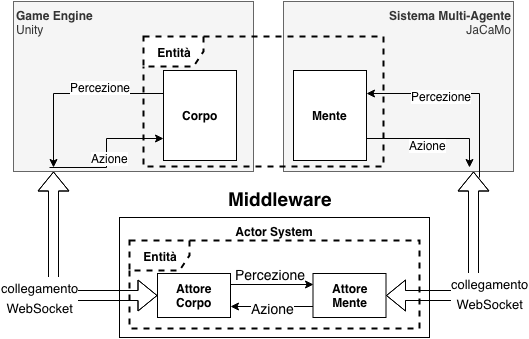
\includegraphics[width=\textwidth]{figures/Synapsis.png}
\caption{Design architetturale}
\end{figure}

Dallo schema è possibile notare come vengono utilizzate le tecnologie precedentemente illustrate:
\begin{itemize}
    \item La Game Engine Unity è adatta ad ospitare il corpo di una generica entità;
    \item JaCaMo è adatto ad ospitare la mente di una generica entità;
    \item Il framework Play viene utilizzato per realizzare il middleware che collega i due sistemi;
    \item La reale connessione viene creata attraverso il protocollo WebSocket integrabile a JaCaMo, Unity e nativamente supportato nel framework Play.
\end{itemize}

Questa soluzione permette a mente e corpo di scambiarsi informazioni, anche se computazionalmente risiedono in sistemi separati, lasciando intatte funzionalità e astrazioni presenti nel Sistema Multi-Agente e nella Game Engine.

\medskip

Con Unity viene "fisicamente" realizzato il corpo di una generica entità: utilizzando il concetto di GameObject ed attraverso i componenti, quali Collidere, Rigibody e script contenenti il collegamento WebSocket, è possibile dotare il corpo di funzionalità adatte a percepire l'ambiente. Ad esempio, in caso di contatto/urto con un diverso oggetto in scena, esso è capace di avvertire l'evento ed inviare alla mente una percezione del tipo \textit{"toccato(nome\_entità\_toccata)"}. 

\medskip

Attraverso Jason viene realizzata la mente dell'entità utilizzando il concetto di agente unito ad un artefatto. Ciò permette di rappresentare il corpo dell'entità all'interno del MAS, interfacciandosi alla GE tramite l'artefatto che contiene la connessione WebSocket. Ad esempio, se la mente vuole far eseguire al corpo una determinata azione è sufficiente che utilizzi l'artefatto collegato per inviare un'azione del tipo \textit{vai\_a (posizione)};

\section{Scenario d'esempio}

Per meglio comprendere l'architettura di sistema appena descritta, e le interazioni tra i suoi componenti costituenti, si prende a riferimento uno scenario d'esempio chiamato "recycling robots". Come si può intuire dal nome, la scena contiene dei robot, i quali hanno il compito di riciclare la spazzatura presente nell'ambiente portandola in un bidone.

\medskip

Il compito generale di un robot è divisibile in un ciclo di sotto-obiettivi, ad esempio:
\begin{enumerate}
    \item Cercare la spazzatura;
    \item Andare verso la spazzatura trovata;
    \item Prendere la spazzatura appena raggiunta;
    \item Cercare il bidone
    \item Andare verso il bidone trovato
    \item Riciclare la spazzatura
\end{enumerate}

Utilizzando il formalismo di Jason, i sotto-obiettivi elencati sono associabili a dei \textit{"plans"} di un agente. Al di fuori del primo plan (Cercare la spazzatura), normalmente attivato dal \textit{"goal"} principale presente nell'agente, i successivi possono essere attivati da una percezione ricevuta dall'agente. Ad esempio, in risposta alla ricerca del bidone è possibile notificare la scoperta di un bidone nelle vicinanze e, di conseguenza, fare in modo che l'agente utilizzi il plan "Andare verso il bidone trovato".

\begin{figure}[H]
\centering
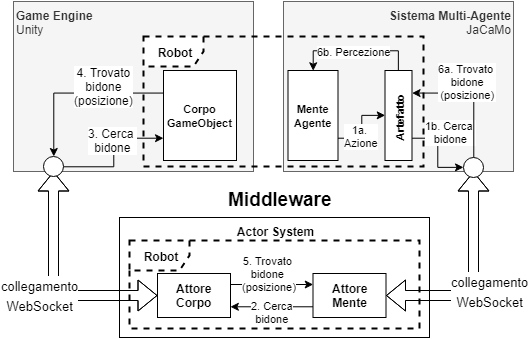
\includegraphics[width=0.7\textwidth]{figures/Esempio.png}
\caption{Esempio di comunicazione tra mente e corpo}
\end{figure}

L'immagine mostra il flusso ordinato di interazioni atteso per l'esempio appena descritto. La mente per svolgere il plan \textit{"Cercare il bidone"} vuole inviare al proprio corpo l'azione \textit{"Cerca bidone"}. Il trasferimento del messaggio avviene attraverso l'artefatto personale dell'agente\footnote{previa associazione dei due}, in possesso del canale WebSocket collegato al middleware, dove è presente un'operazione che invia il messaggio al middleware.

\medskip 

L'attore mente presente nel middleware alla ricezione delle infomazioni da inviare al corpo, inoltra le stesse all'attore corpo che è l'unico possessore del riferimento all'entità corpo presente su Unity e, quindi, in grado di inoltrare il messaggio al corpo "reale". Quando su Unity l'entità corpo (GameObject) riceve il messaggio, attraverso il canale WebSocket, attua l'azione a lui richiesta e risponde alla mente inviando la percezione generata.

\medskip

A questo punto la percezione viene mandata al middleware, più precisamente all'attore "corpo" che a sua volta la inoltrerà all'attore "mente", che la invierà poi all'artefatto collegato, sempre tramite WebSocket.

\medskip

L'artefatto, alla ricezione della percezione, aggiunge quest'ultima alle sue proprietà osservabili che, automaticamente, aggiorneranno la BeliefBase dell'agente. L'ultimo passaggio rappresenta il punto cruciale per completare il collegamento tra corpo e mente dato che in questa maniera l'agente ha ricevuto la percezione dal proprio corpo. 

\medskip

Si intende inoltre lasciare aperta la possibilità, da parte del corpo, di inviare percezioni non come reazione ad azioni eseguite dalla mente, dato che il collegamento WebSocket, una volta effettuato, rimane attivo per tutta la durata di vita dell'entità. Ad esempio, in caso di contatto con un oggetto nella scena Unity, il corpo deve essere in grado di mandare una percezione del tipo \textit{"toccata(nome\_oggetto,posizione)"} alla propria mente senza bisogno di stimoli.

\medskip

Per concludere, il lavoro di attività propedeutica ha permesso di acquisire la necessaria conoscenza e dimestichezza con i concetti e le tecnologie da utilizzare per la successiva realizzazione del middleware in fase di tesi.
 


%%%%%%%%%%%%%%%%%%%%%%%%%
% inizio parte finale del documento
%
% eventuali appendici, bibliografia obbligatoria,
% eventuale lista delle tabelle e delle figure (nel caso decommentare la riga con i comandi \listoffigures e \listoftables)
%%%%%%%%%%%%%%%%%%%%%%%%%
\backmatter

%\listoftodos[Lista Note]
\listoffigures
%\listoftables
%\lstlistoflistings
\bibliography{biblio}
\bibliographystyle{abbrv}

% chiusura del documento
\end{document}
